\subsection{UC11 - Visualizzazione Ore da Consuntivare Rimanenti }
\begin{itemize}
	\item \textbf{Identificativo}: UC11
	\item \textbf{Nome}: Visualizzazione ore da consuntivare rimanenti
	\item \textbf{Descrizione Grafica}:
	\begin{figure}[h]
		\centering
		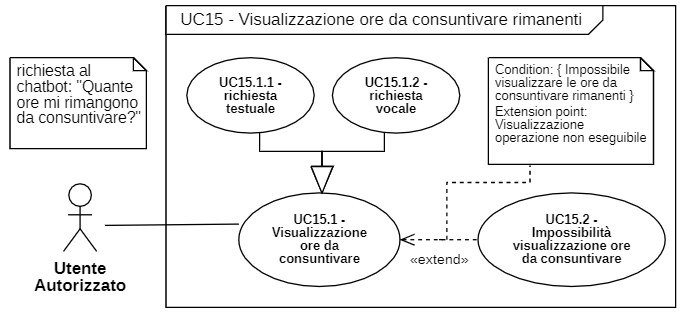
\includegraphics[scale=0.80]{images/UC11.png} 
		\caption{Descrizione grafica caso d'uso UC11}
	 \end{figure}

	\item \textbf{Attori}
	\begin{itemize} 
		\item \textit{Primari}: Utente autorizzato
		\item \textit{Secondari}: Non presenti
	\end{itemize}
	\item \textbf{Descrizione}: L'utente visualizza le ore rimanenti da consuntivare nella giornata.
	\item \textbf{Precondizione}: L'utente richiede di vedere quante ore gli rimangono da consuntivare.
	\item \textbf{Postcondizione}: Il chatbot notifica il numero rimanente di ore da consuntivare nella giornata.
	\item \textbf{Scenario principale}: \begin{enumerate}
		\item L'utente invia una richiesta del tipo: `Quante ore mi rimangono da consuntivare?';
		\item Chatbot comunica: `Hai ancora X ore da consuntivare'.
	\end{enumerate}
\end{itemize}

\subsubsection{UC11.1 - Visualizzazione Ore da Consuntivare}
\begin{itemize}
	\item \textbf{Identificativo}: UC11.1
	\item \textbf{Nome}: Visualizzazione ore da consuntivare
	\item \textbf{Descrizione Grafica}: (Approfondita in UC11)
	\item \textbf{Attori}
	\begin{itemize} 
		\item \textit{Primari}: Utente autorizzato
		\item \textit{Secondari}: Non presenti
	\end{itemize}
	\item \textbf{Descrizione}: L'utente comunica al chatbot di voler vedere le ore rimanenti.
	\item \textbf{Precondizione}: L'utente richiede la visualizzazione delle ore rimanenti da consuntivare.
	\item \textbf{Postcondizione}: Il chatbot notifica il numero rimanente di ore da consuntivare nella giornata.
	\item \textbf{Scenario principale}: Dopo che l'utente invia la richiesta il chatbot visualizza il numero di ore da consuntivare.
\end{itemize}

\subsubsection{UC11.1.1 - Richiesta Testuale}
\begin{itemize}
	\item \textbf{Identificativo}: UC11.1.1
	\item \textbf{Nome}: Richiesta testuale
	\item \textbf{Descrizione Grafica}: (Approfondita in UC11)
	\item \textbf{Attori}
	\begin{itemize} 
		\item \textit{Primari}: Utente autorizzato
		\item \textit{Secondari}: Non presenti
	\end{itemize}
	\item \textbf{Descrizione}: L'utente comunica al chatbot tramite input testuale di voler vedere le ore rimanenti.
	\item \textbf{Precondizione}: L'utente vuole inviare la richiesta di visualizzazione delle ore rimanenti.
	\item \textbf{Postcondizione}: L'utente inserisce la richiesta in formato testuale.
	\item \textbf{Scenario principale}:
	\begin{enumerate}
		\item L'utente vuole visualizzare le ore da consuntivare;
		\item L'utente inserisce tramite input testuale la richiesta.
	\end{enumerate}
\end{itemize}

\subsubsection{UC11.1.2 - Richiesta Vocale}
\begin{itemize}
	\item \textbf{Identificativo}: UC11.1.2
	\item \textbf{Nome}: Richiesta vocale
	\item \textbf{Descrizione Grafica}: (Approfondita in UC11)
	\item \textbf{Attori}
	\begin{itemize} 
		\item \textit{Primari}: Utente autorizzato
		\item \textit{Secondari}: Non presenti
	\end{itemize}
	\item \textbf{Descrizione}: L'utente comunica al chatbot tramite input vocale di voler vedere le ore rimanenti.
	\item \textbf{Precondizione}: L'utente vuole inviare la richiesta di visualizzazione delle ore rimanenti.
	\item \textbf{Postcondizione}: L'utente inserisce la richiesta in formato vocale.
	\item \textbf{Scenario principale}:
	\begin{enumerate}
		\item L'utente vuole visualizzare le ore da consuntivare;
		\item L'utente inserisce tramite input vocale la richiesta.
	\end{enumerate}
\end{itemize}

\subsubsection{UC11.2 - Impossibilità Visualizzazione Ore da Consuntivare}
\begin{itemize}
	\item \textbf{Identificativo}: UC11.2
	\item \textbf{Nome}: Impossibilità visualizzazione ore da consuntivare
	\item \textbf{Descrizione Grafica}: (Approfondita in UC11)
	\item \textbf{Attori}
	\begin{itemize} 
		\item \textit{Primari}: Utente autorizzato
		\item \textit{Secondari}: Non presenti
	\end{itemize}
	\item \textbf{Descrizione}: L'utente comunica al chatbot di voler vedere le ore rimanenti ma viene restituito un messaggio d'errore.
	\item \textbf{Precondizione}: L'utente richiede la visualizzazione delle ore rimanenti da consuntivare.
	\item \textbf{Postcondizione}: il chatbot risponde con un messaggio d'errore indicando l'impossibilità di effettuare l'operazione.
	\item \textbf{Scenario principale}: L'utente richiede di vedere le ore da consuntivare, ma gli viene negato e visualizza un messaggio d'errore.
\end{itemize}
\newpage